\documentclass[aspectratio=169,9pt]{beamer}
% Beamer layout
\setbeamersize{text margin left=0.4cm, text margin right=0.2cm}

% Math & fonts
\usepackage{amsmath,amssymb}
\usepackage{mathpazo}   % Palatino text + math

% Tables & units
\usepackage{booktabs}
\usepackage{siunitx}

% TikZ (one load, all libs)
\usepackage{tikz}
\usetikzlibrary{arrows.meta,calc,positioning,shapes.geometric,shapes.misc}

% Algorithms
\usepackage{algorithm}
\usepackage[noend]{algpseudocode}
\usepackage{float}

% Media
\usepackage{multimedia}
\usepackage{animate}

% Bibliography
\usepackage{natbib}


\newcommand{\shortdate}{\the\month-\the\day}
\graphicspath{{../../figures/.}}


\definecolor{cardinalred}{RGB}{140,21,21}
\definecolor{coolgray}{RGB}{77,79,83}
\definecolor{black}{RGB}{0,0,0}
\definecolor{beige}{RGB}{210,194,149}
\definecolor{darkbeige}{RGB}{179,153,93}
\definecolor{darkcardinal}{RGB}{94,48,50}
\definecolor{lightcardinal}{RGB}{141,60,30}
\definecolor{darkpurple}{RGB}{83,40,79}
\definecolor{darkcyan}{RGB}{0,124,146}
\definecolor{skyblue}{RGB}{0,152,219}
\definecolor{treegreen}{RGB}{0,155,118}
\definecolor{darkorange}{RGB}{168,101,12}
\definecolor{beigegray}{RGB}{95,87,79}
\definecolor{boxgray}{RGB}{238,235,233}
\definecolor{footergray}{RGB}{199,209,197}



\mode<presentation>

\setbeamercolor*{palette primary}{use=structure,fg=white,bg= cardinalred}
\setbeamercolor*{palette secondary}{use=structure,fg=white,bg= coolgray}
\setbeamercolor*{palette tertiary}{use=structure,fg=white,bg= darkcardinal}
\setbeamercolor*{palette quaternary}{fg=white,bg= darkbeige}

\setbeamercolor*{sidebar}{use=structure,bg= beige}
\setbeamercolor*{footer}{use=structure,bg= footergray,fg=darkcardinal}
  
\setbeamercolor*{palette sidebar primary}{use=structure,fg=structure.fg!10}
\setbeamercolor*{palette sidebar secondary}{fg=white}
\setbeamercolor*{palette sidebar tertiary}{use=structure,fg=structure.fg!50}
\setbeamercolor*{palette sidebar quaternary}{fg=white}

\setbeamercolor*{titlelike}{parent=palette primary}
\setbeamercolor*{foot line}{parent=palette secondary}

\setbeamercolor*{separation line}{}
\setbeamercolor*{fine separation line}{}

\setbeamercolor{itemize item}{fg=cardinalred}
\setbeamercolor{itemize subitem}{fg=cardinalred}
\setbeamercolor{itemize subsubitem}{fg=cardinalred}
\setbeamercolor{enumerate item}{fg=cardinalred}
\setbeamercolor{enumerate subitem}{fg=cardinalred}
\setbeamercolor{enumerate subsubitem}{fg=cardinalred}
\setbeamercolor{description item}{fg=cardinalred}

\setbeamertemplate{bibliography item}[text]
\setbeamertemplate{frametitle continuation}[from second]
\setbeamercolor{bibliography entry title}{fg=black}
\setbeamercolor{bibliography entry author}{fg=black}
\setbeamercolor*{bibliography entry location}{fg=black}
\setbeamercolor*{bibliography entry note}{fg=black}

\renewcommand*{\bibfont}{\small}
\setbeamertemplate{navigation symbols}{}

\setbeamerfont{footnote}{size=\tiny}

\mode
<all>
\definecolor{cardinalred}{RGB}{140,21,21}
%--- Custom footline
\setbeamertemplate{footline}{%
\begin{beamercolorbox}[wd=\paperwidth,ht=4ex,dp=2.5ex]{}
    \centering
    \makebox[0.32\paperwidth][l]{\scriptsize\texttt{Pipe. \shortdate}}
    \makebox[0.32\paperwidth][c]{\scriptsize\texttt{$^{\dag}$masseyj@stanford.edu}}
    \makebox[0.32\paperwidth][r]{\scriptsize\insertframenumber/\inserttotalframenumber}
  \end{beamercolorbox}
}
\usepackage{algorithm}
\usepackage[noend]{algpseudocode}
\usetikzlibrary{arrows.meta,shapes.geometric,shapes.misc,positioning}

\tikzset{
  >={Stealth},
  proc/.style = {rectangle, rounded corners, draw, align=left, minimum height=8mm, text width=35mm, align=center},
  meas/.style    = {trapezium, trapezium left angle=70, trapezium right angle=110, draw, align=left, minimum height=8mm, text width=19mm, align=center},
  decision/.style = {diamond, aspect=2.2, draw, align=center, inner xsep=1.2ex, inner ysep=1ex, text width=2cm},
  smldec/.style = {diamond, aspect=2.2, draw, align=center, inner xsep=1.2ex, inner ysep=1ex, text width=19mm},
  terminator/.style = {ellipse, draw, align=center, minimum height=8mm, minimum width=16mm},
  line/.style  = {->, line width=0.6pt}
}


%--- Title info
\title{Pressure measurements}
\author{JMO Massey$^{\dag}$, F Cabrera-Booman, T Jaroslawski, JC Klewicki, BJ McKeon}
\institute{Center for Turbulence Research \\ Stanford University}
% \thanks{This work was supported by DARPA under the CHAOS program}
\date{\today}

\begin{document}

%--- Title page
\begin{frame}
    \setcounter{framenumber}{0}
    \titlepage
    \vfill
    {\scriptsize \centering Thanks to DARPA for funding this work.\par}
\end{frame}

\begin{frame}
  \frametitle{POA}
  \begin{enumerate}
    \item Focus on 50psi ph calibration signals
    \item Show the raw signals
    \begin{itemize}
        \item Show loglog for 3 cases.
        \item No noise, w. background noise, white noise ?
    \end{itemize}
    \item Show the spectra
    \item Show with HP filtering
    \item Apply transfer function and show the TF
    \item Determine whether a LP filter can be applied at $f=2kHz$
    \begin{itemize}
        \item $T^+\equiv T u_\tau^2/\nu$
        \item at 50psi $Re_\tau\approx 5000$ $u_\tau\approx 0.51$, $\nu\approx 1.43$
        \item $T^+=20 \to f=948Hz$
    \end{itemize}
    \item 
  \end{enumerate}
\end{frame}

\begin{frame}
  \frametitle{Raw signals}
  \begin{figure}
    \centering
    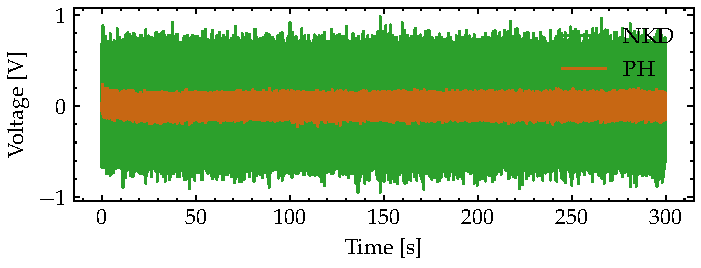
\includegraphics[width=0.4\textwidth]{sanity/50psi/PH-NKD/calib_ts_signals_50psi_nonoise.pdf}
    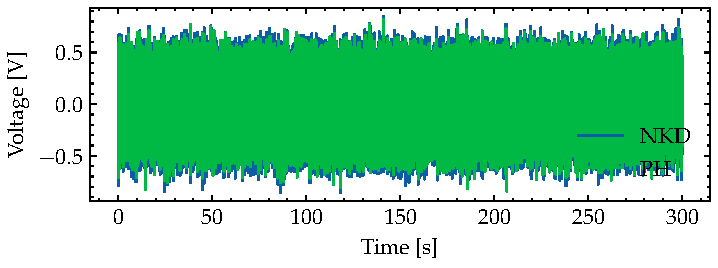
\includegraphics[width=0.4\textwidth]{sanity/50psi/PH-NKD/calib_ts_signals_50psi_noise.pdf}
    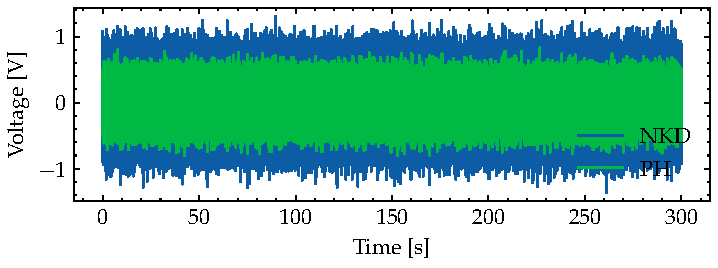
\includegraphics[width=0.4\textwidth]{sanity/50psi/PH-NKD/calib_ts_signals_50psi_noiseWN.pdf}
  \end{figure}
  \textbf{Top left:} white noise, \textbf{top right:} \emph{only} facility noise, \textbf{bottom:} white noise + facility noise
\end{frame}

\begin{frame}
  \frametitle{Raw Spectra}
  \begin{figure}
    \centering
    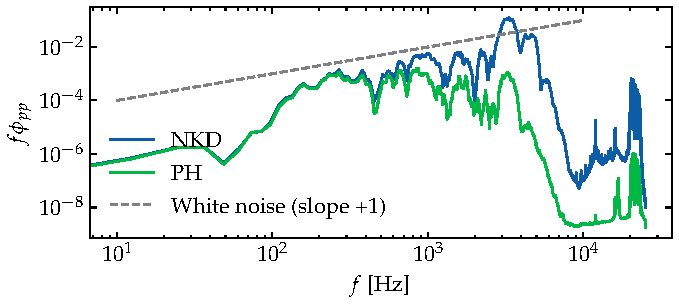
\includegraphics[width=0.4\textwidth]{sanity/50psi/PH-NKD/calib_spectra_50psi_nonoise.pdf}
    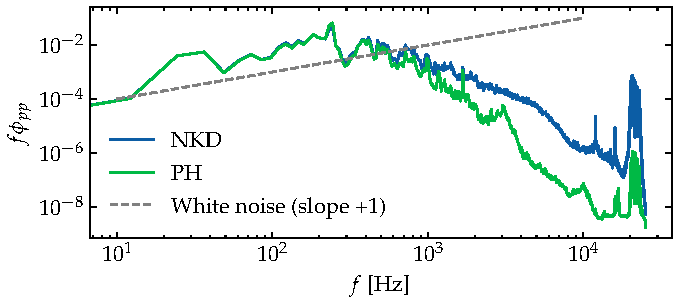
\includegraphics[width=0.4\textwidth]{sanity/50psi/PH-NKD/calib_spectra_50psi_noise.pdf}
    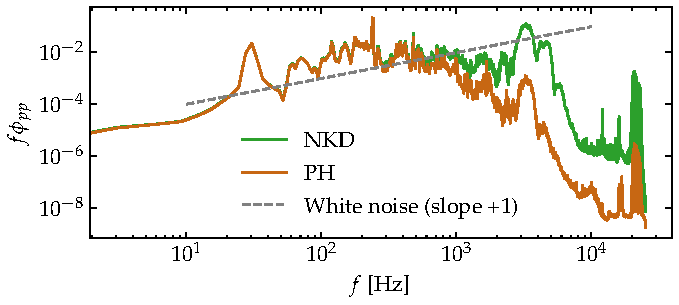
\includegraphics[width=0.4\textwidth]{sanity/50psi/PH-NKD/calib_spectra_50psi_noiseWN.pdf}
  \end{figure}
%   Tomek to explain \textbf{top left:} \textbf{top right:} \textbf{bottom:}
\end{frame}

\begin{frame}
  \frametitle{Does the noise add up?}
    \centering
    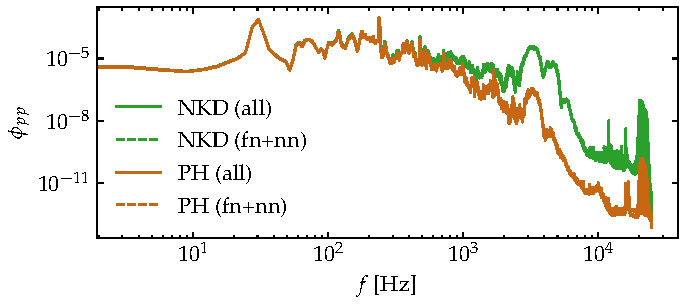
\includegraphics[width=0.8\textwidth]{sanity/50psi/PH-NKD/calib_spectra_50psi_nkd_fn_plus_nn.pdf}
\end{frame}

\begin{frame}
    \frametitle{Do the TFs look reasonably similar?}
        \centering
        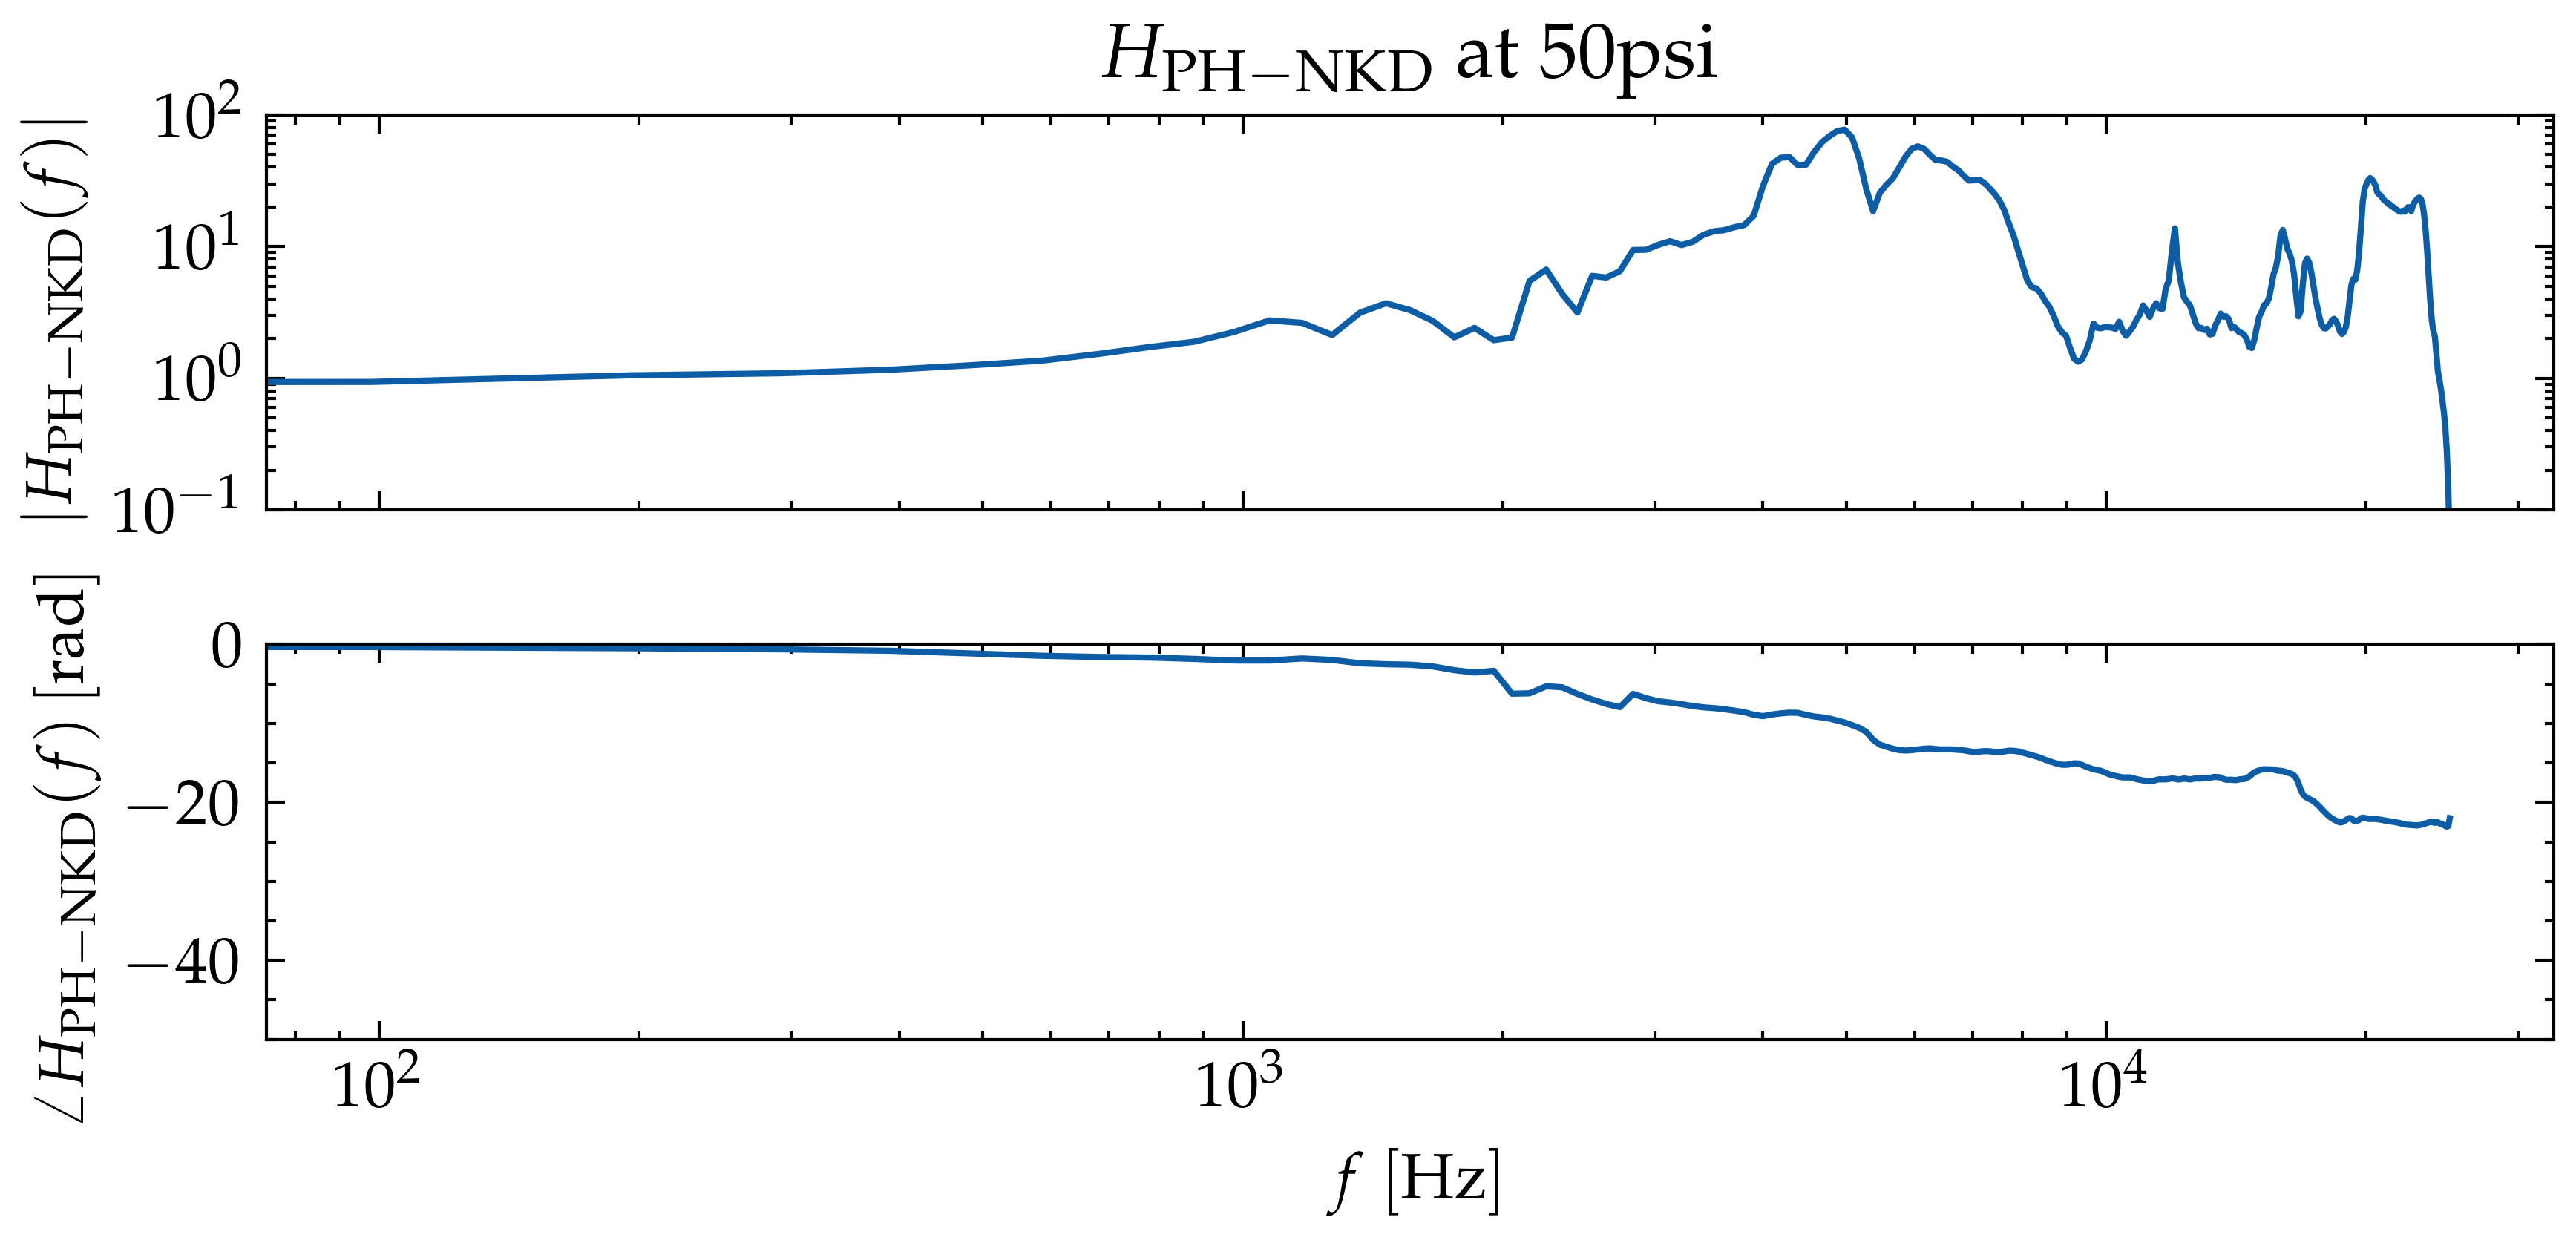
\includegraphics[width=0.4\textwidth]{sanity/50psi/PH-NKD/H_50psi_nn.png}
        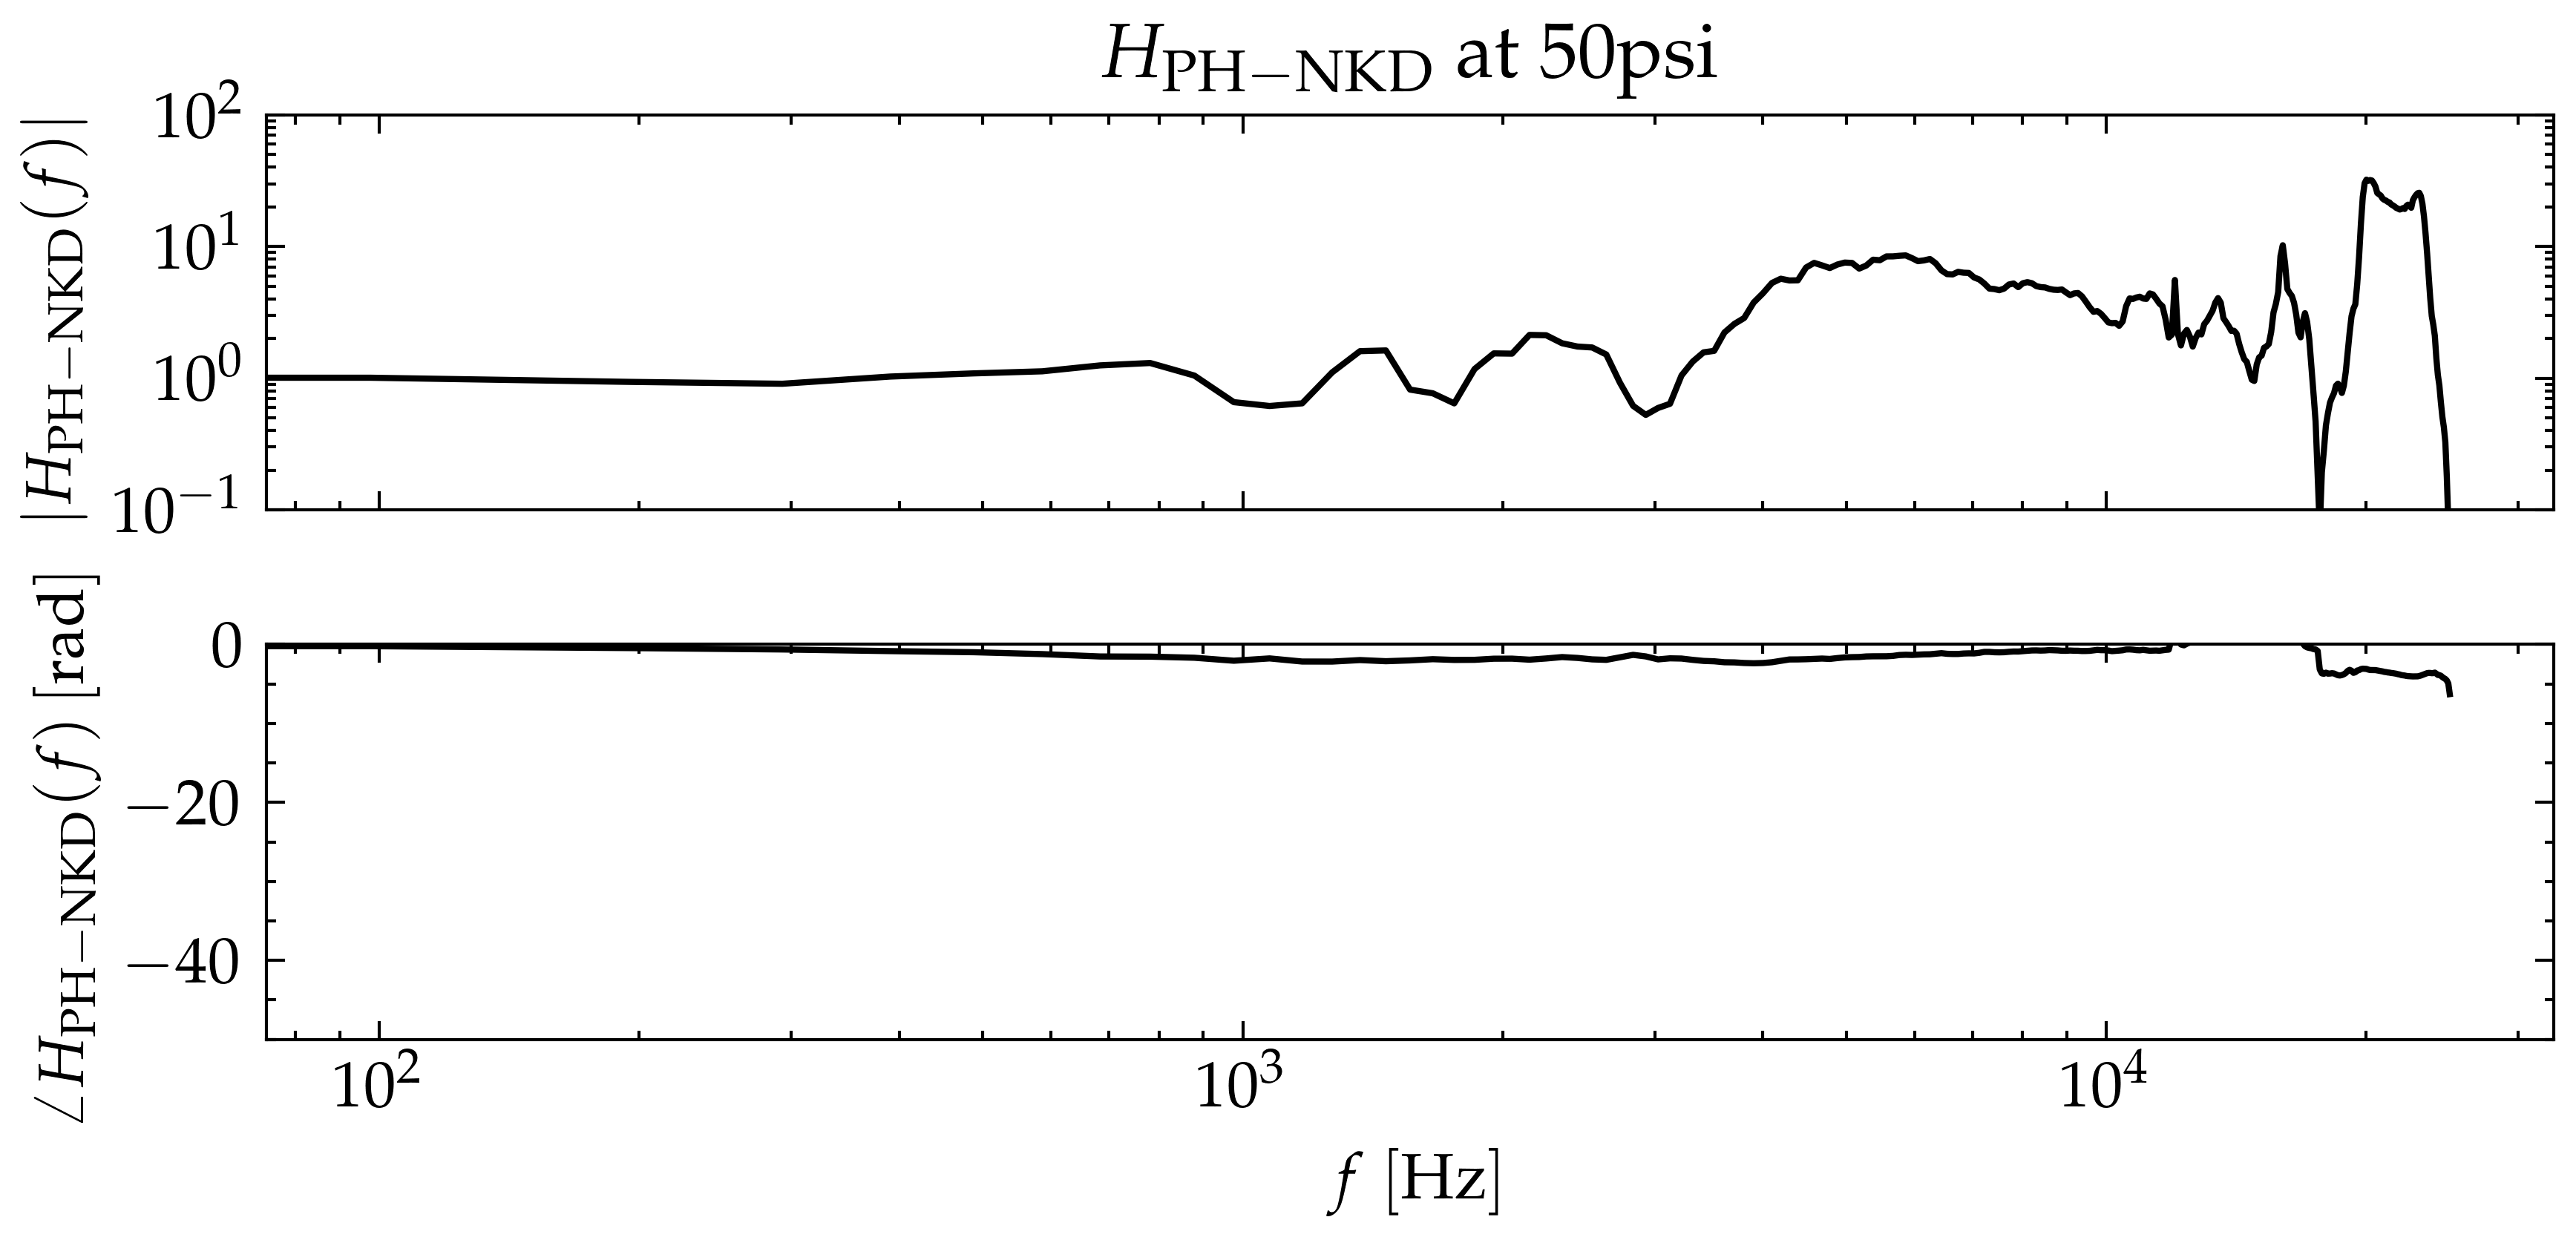
\includegraphics[width=0.4\textwidth]{sanity/50psi/PH-NKD/H_50psi_fn.png}
        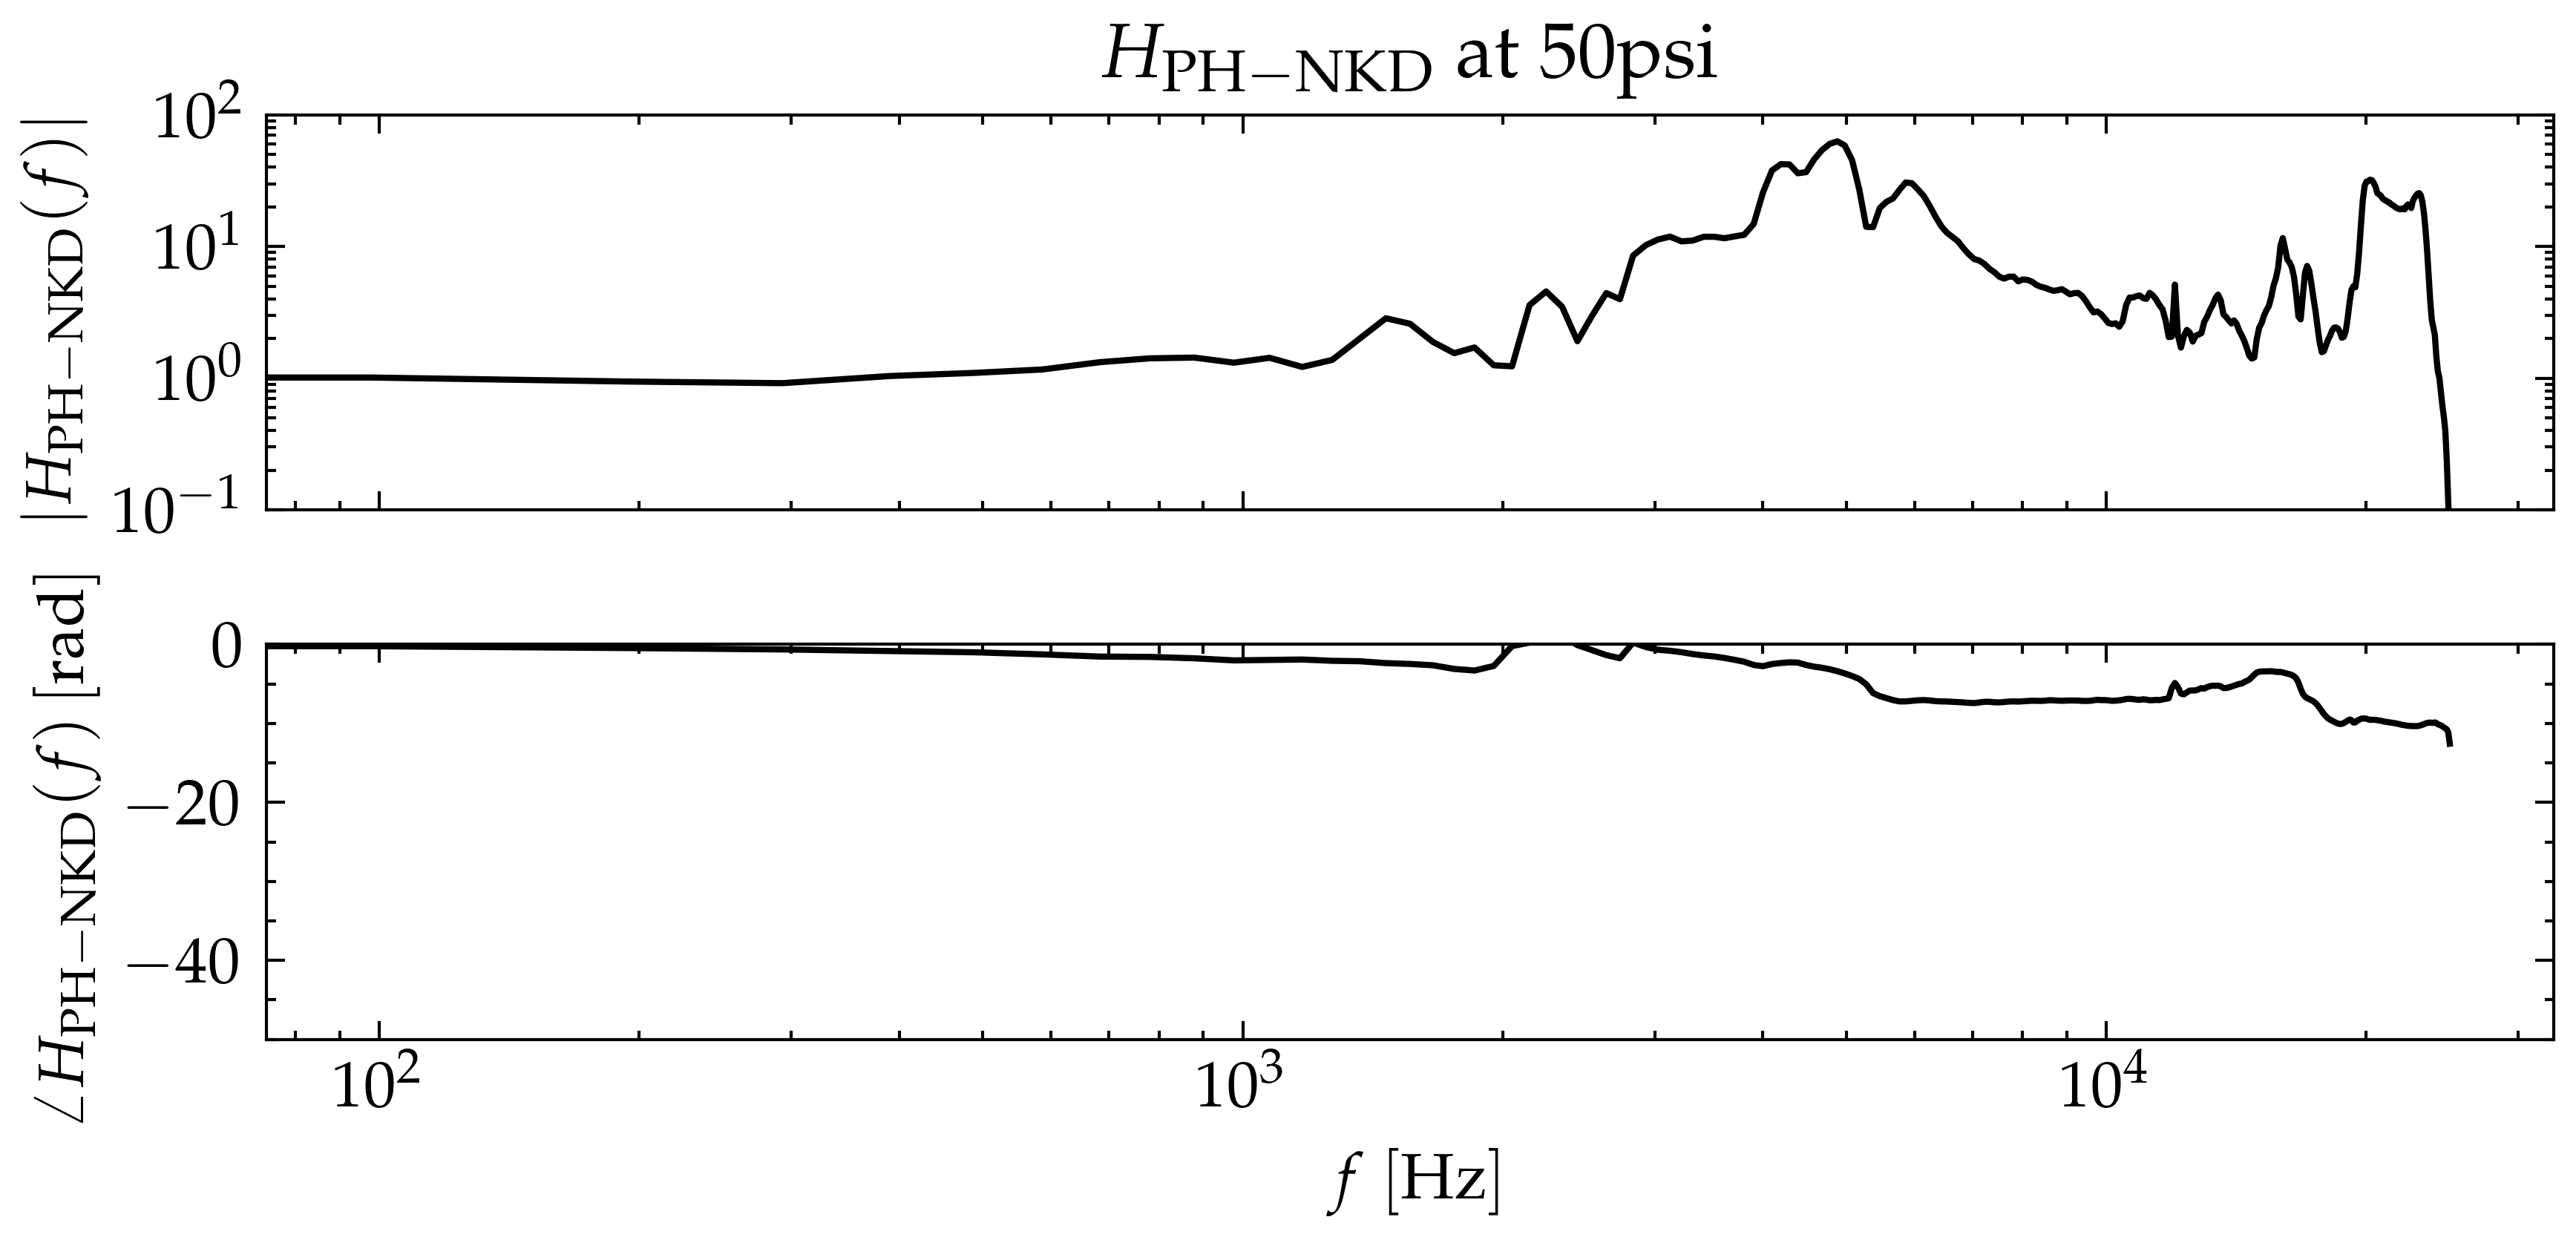
\includegraphics[width=0.4\textwidth]{sanity/50psi/PH-NKD/H_50psi_an.png}
\end{frame}

\begin{frame}
    \frametitle{TF reconstructed spectra}
        \centering
        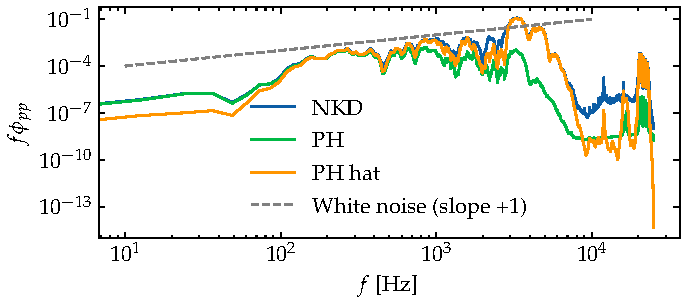
\includegraphics[width=0.4\textwidth]{sanity/50psi/PH-NKD/calib_spectra_50psi_nn_recon.pdf}
        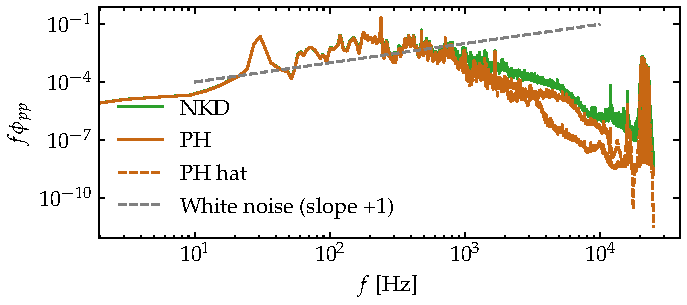
\includegraphics[width=0.4\textwidth]{sanity/50psi/PH-NKD/calib_spectra_50psi_fn_recon.pdf}
        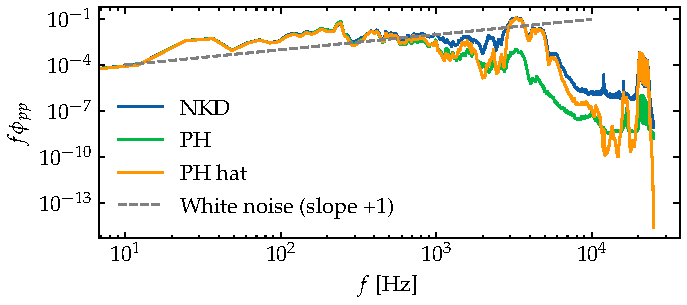
\includegraphics[width=0.4\textwidth]{sanity/50psi/PH-NKD/calib_spectra_50psi_an_recon.pdf}
\end{frame}

\begin{frame}
    \frametitle{Spectra w. HP \& LP filter}
    Filter at 0.1Hz and 2kHz corresponding to LP cutoff of $T^+=10$ at 50psi
        \centering
        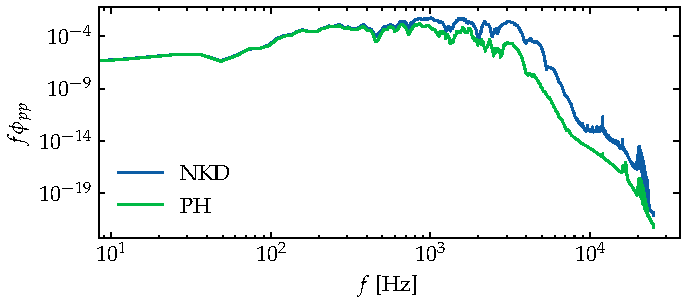
\includegraphics[width=0.4\textwidth]{sanity/50psi/PH-NKD/calib_spectra_50psi_nn_filt.pdf}
        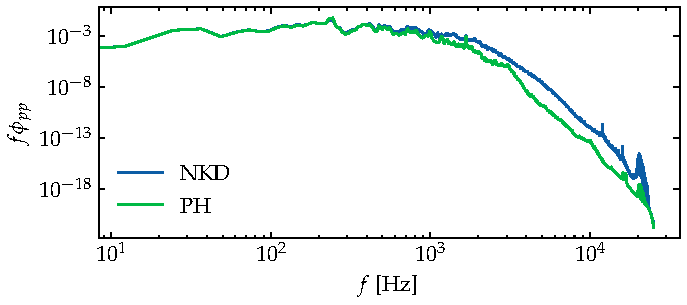
\includegraphics[width=0.4\textwidth]{sanity/50psi/PH-NKD/calib_spectra_50psi_fn_filt.pdf}
        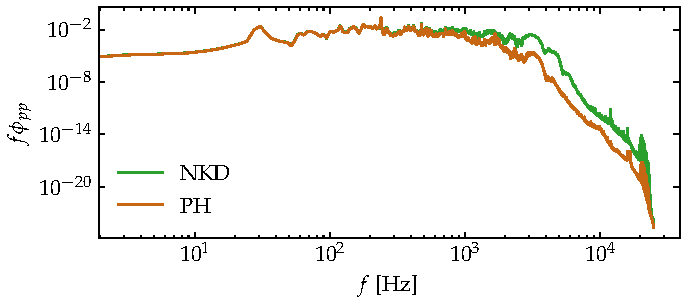
\includegraphics[width=0.4\textwidth]{sanity/50psi/PH-NKD/calib_spectra_50psi_an_filt.pdf}
\end{frame}

\begin{frame}
    \frametitle{Do the TFs look reasonably similar after filtering?}
        \centering
        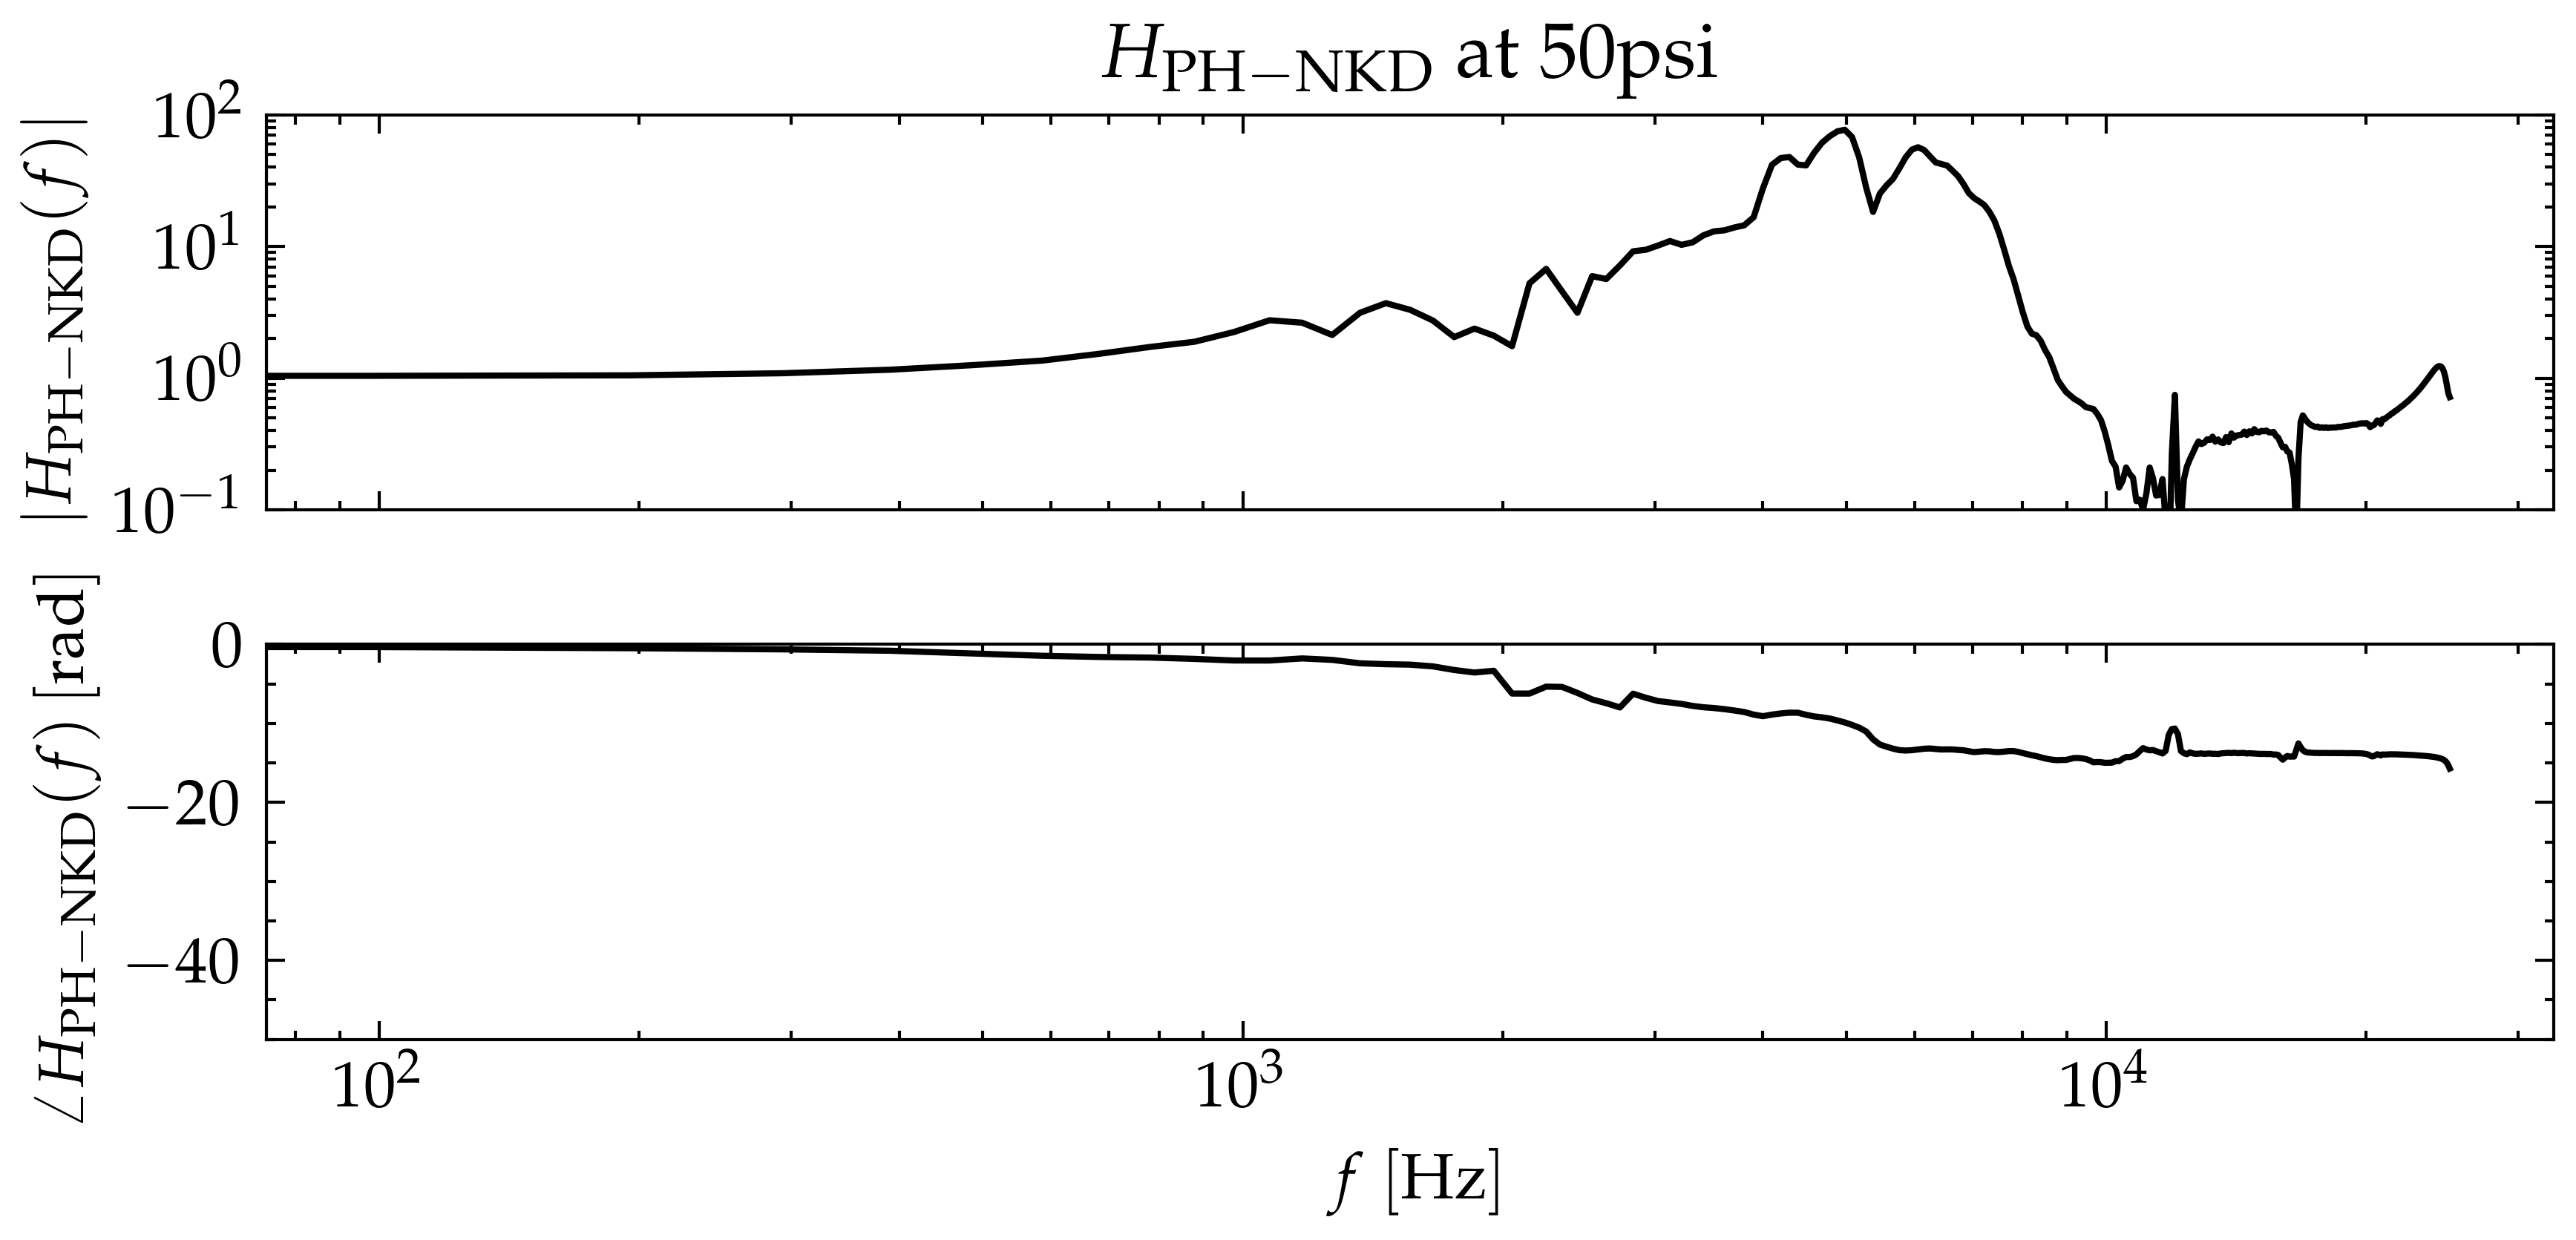
\includegraphics[width=0.4\textwidth]{sanity/50psi/PH-NKD/H_50psi_nn_filt.png}
        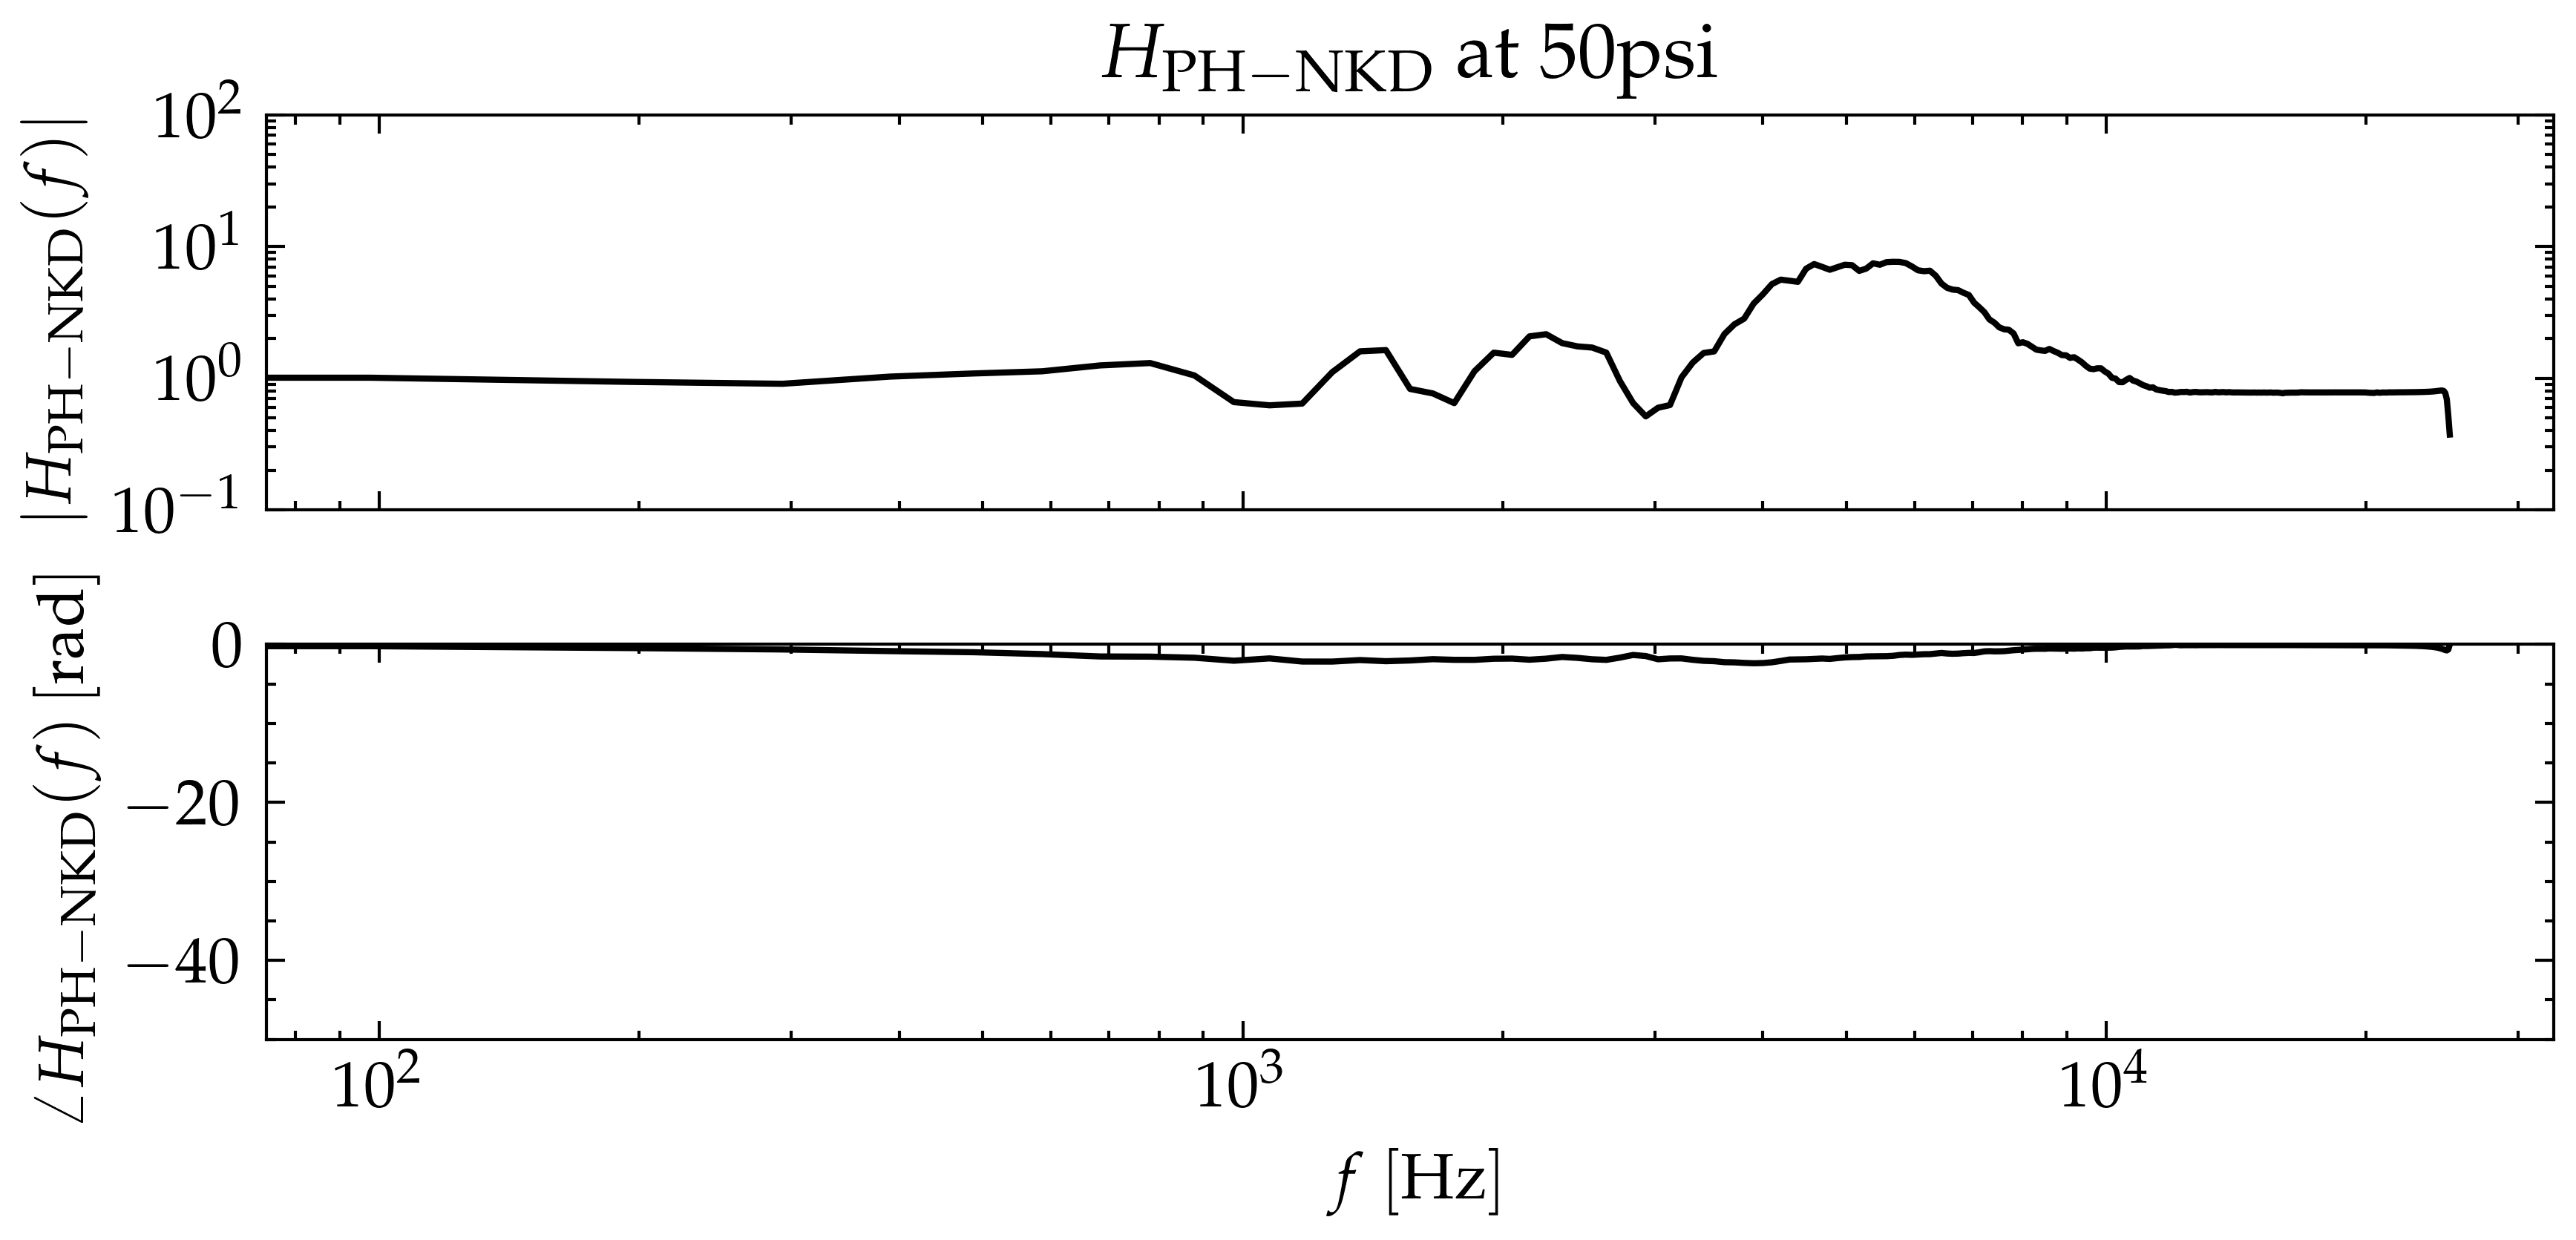
\includegraphics[width=0.4\textwidth]{sanity/50psi/PH-NKD/H_50psi_fn_filt.png}
        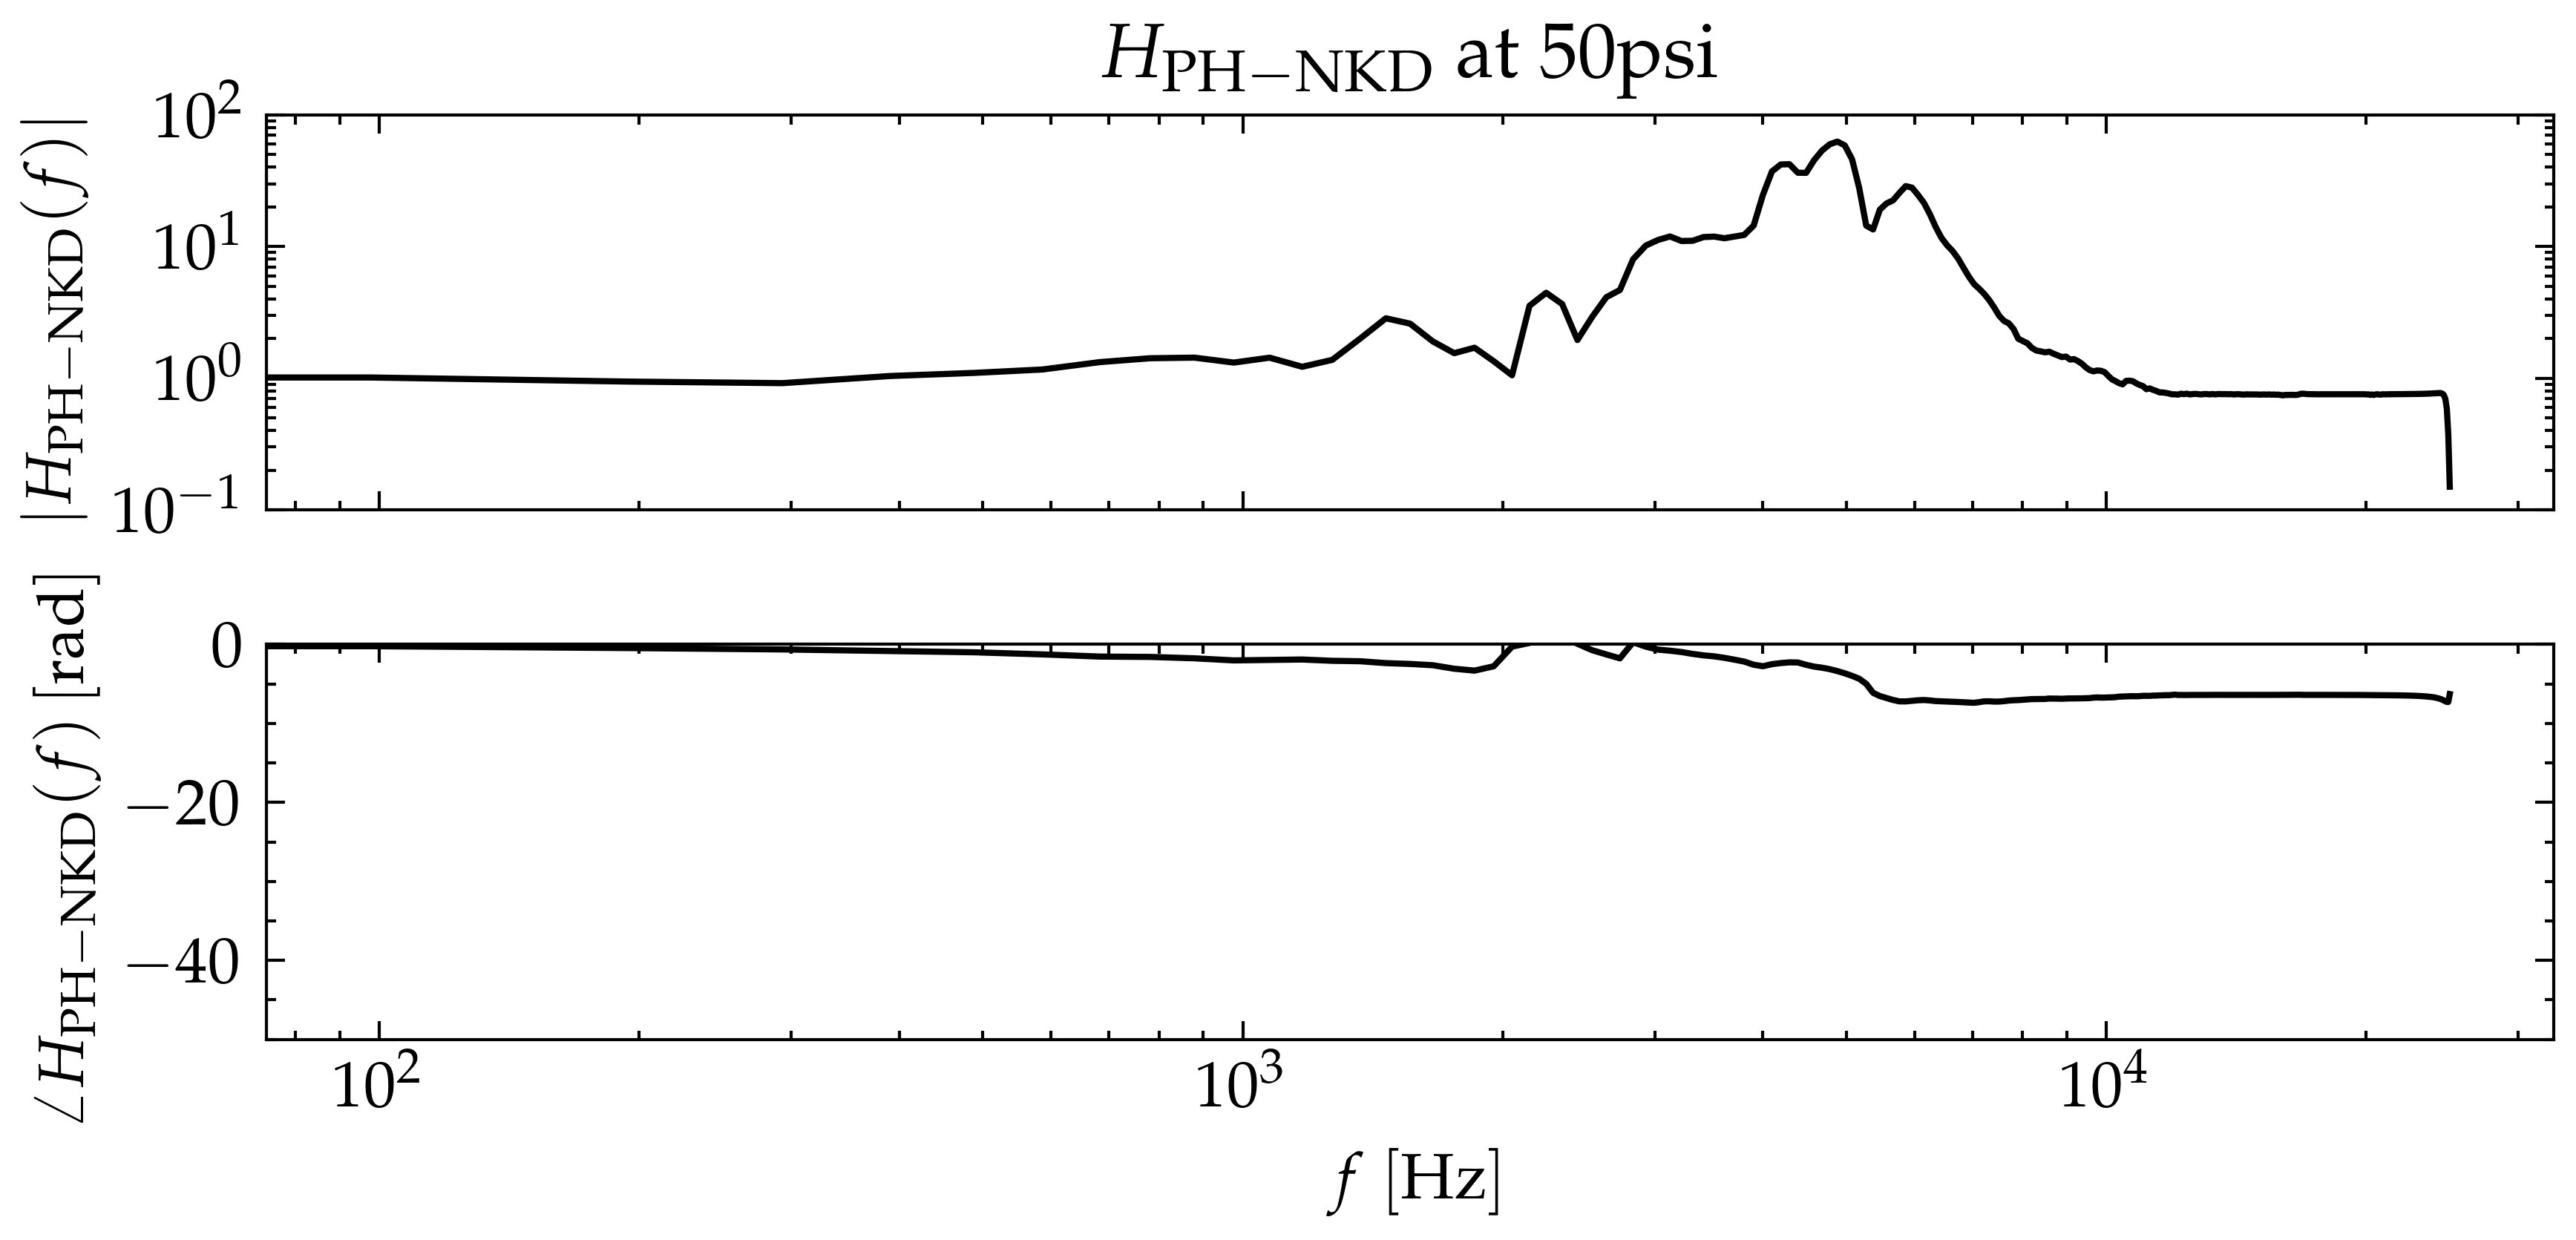
\includegraphics[width=0.4\textwidth]{sanity/50psi/PH-NKD/H_50psi_an_filt.png}
\end{frame}

\begin{frame}
    \frametitle{TF reconstructed spectra with HP \& LP filter}
        \centering
        \includegraphics[width=0.4\textwidth]{sanity/50psi/PH-NKD/calib_spectra_50psi_nn_recon_filt.pdf}
        \includegraphics[width=0.4\textwidth]{sanity/50psi/PH-NKD/calib_spectra_50psi_fn_recon_filt.pdf}
        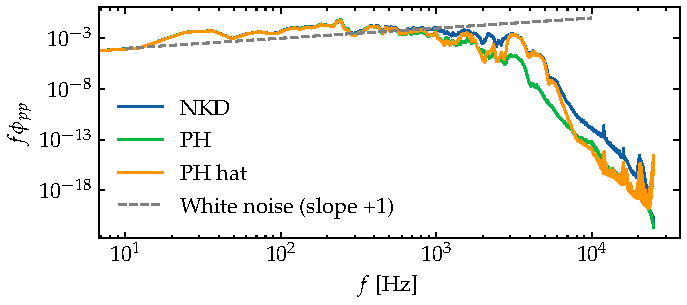
\includegraphics[width=0.4\textwidth]{sanity/50psi/PH-NKD/calib_spectra_50psi_an_filt_recon.pdf}
\end{frame}





\end{document}
